\documentclass[11pt,a4paper]{article}
\usepackage[margin=23mm]{geometry}
\usepackage{fontspec}
\usepackage{amsmath,amssymb,booktabs,graphicx}
\usepackage[hidelinks]{hyperref}
\setmainfont{Malgun Gothic}
\XeTeXlinebreaklocale "ko"
\XeTeXlinebreakskip=0pt plus 1pt
\renewcommand{\refname}{참고문헌 및 자료 출처}
\setlength{\parindent}{0pt}
\setlength{\parskip}{5pt}
\newcommand{\FirstDate}{2022-04-01}
\newcommand{\LastDate}{2025-12-31}
\newcommand{\SampleSize}{941}
\newcommand{\CurveCount}{998}
\newcommand{\ExampleDate}{2025-12-31}
\newcommand{\MeanParRMSE}{1.53}
\newcommand{\MeanZeroRMSE}{0.67}
\newcommand{\CurveMinDiscount}{0.214}
\newcommand{\NegativeForwardDates}{0}
\newcommand{\MedianTurns}{4}
\newcommand{\WeakForwardShift}{1.67}
\newcommand{\StrongForwardShift}{3.23}
\newcommand{\FitError}{3.05e-16}
\newcommand{\RiccatiError}{2.26e-11}
\newcommand{\InitialSigma}{0.53}
\newcommand{\IefDistributionCount}{48}
\newcommand{\TltDistributionCount}{48}
\newcommand{\ModelDelta}{4.53}
\newcommand{\ModelLow}{3.23}
\newcommand{\ModelHigh}{5.78}
\newcommand{\MatchedDelta}{0.02}
\newcommand{\MatchedLow}{-0.19}
\newcommand{\MatchedHigh}{0.27}
\newcommand{\NssSplineParMedian}{2.064}
\newcommand{\NssParMedian}{3.482}
\newcommand{\NssSplineZeroMedian}{0.674}
\newcommand{\NssZeroMedian}{6.743}
\newcommand{\NssBoundDates}{183}
\newcommand{\NssHjbSplineSd}{23.759}
\newcommand{\NssHjbSplineTurnover}{190.431}
\newcommand{\NssHjbNssSd}{23.521}
\newcommand{\NssHjbNssTurnover}{190.442}

\newcommand{\dif}{\mathrm d}
\makeatletter
\let\tableinput\@@input
\makeatother

\title{\textbf{Hull--White 모형을 이용한 IEF--TLT 연속시간 헤징}\\
\large Smoothing Spline과 Nelson--Siegel--Svensson 비교}
\author{금융수학 중간과제}
\date{}

\begin{document}
\maketitle

\section{연구 목적 및 자료}

IEF 1주의 금리위험을 TLT 매도 포지션으로 헤지한다. Smoothing Spline과 Nelson--Siegel--Svensson(NSS)으로 얻은 Yield Curve을 각각 적용하고, 곡선 추정법에 따라 헤지 성과가 얼마나 달라지는지 비교한다. Spline과 NSS는 각각 Reinsch \cite{reinsch}와 Svensson \cite{svensson}을 참고했다.

2022--2025년 미국 재무부의 일별 Par Yield \CurveCount{}개 곡선과 Nasdaq의 IEF·TLT 종가 및 현금 분배금을 사용했다 \cite{treasury,ief,tlt}. 초기 추정 구간을 제외한 손익 평가 기간은 \FirstDate{}부터 \LastDate{}까지 총 \SampleSize{}거래일이다. 두 실험에서 시장가격, 신호 시점, Trading Cost, HJB 파라미터를 동일하게 적용했다. 거래는 신호 다음 거래일 종가에 반영했고, TLT 거래금액의 2\,bp를 비용으로 차감했다.

\section{Interest Rate Model과 Hedging 설정}

\subsection{Hull--White Model과 Forward Curve}

Risk-Neutral Measure에서 Short Rate $r_t$는 다음 식을 따른다. $a$는 Mean-Reversion Speed이고, $\sigma$는 Short-Rate Volatility이다 \cite{hw}.
\[
 \dif r_t=(\theta(t)-ar_t)\dif t+\sigma\dif W_t^{\mathbb Q},
 \qquad
 \theta(t)=\partial_t f(0,t)+af(0,t)
              +\frac{\sigma^2}{2a}(1-e^{-2at}).
\]
만기 $\tau$의 Continuously Compounded Zero Rate를 $z(\tau)$라 하면, Discount Factor는 $P(0,\tau)=e^{-\tau z(\tau)}$이고 Instantaneous Forward Rate는 $f(0,\tau)=z(\tau)+\tau z'(\tau)$이다.

\textbf{Smoothing Spline.} 관측 Par Yield에 Natural Cubic Smoothing Spline을 적합하고, Semiannual Coupon을 기준으로 Discount Factor를 Bootstrap한다. 이 값에서 얻은 Zero-Rate Node $z_i$에 Natural Cubic Smoothing Spline을 다시 적합한다.
\[
 \widehat z=\arg\min_g\left\{\sum_i[z_i-g(\tau_i)]^2
                  +\rho\int[g''(\tau)]^2\dif\tau\right\},
 \qquad f_{\mathrm{Spline}}(0,\tau)=\widehat z(\tau)+\tau\widehat z'(\tau).
\]
두 Spline의 Smoothing Parameter는 Generalized Cross-Validation(GCV)으로 정했다.

\textbf{Nelson--Siegel--Svensson (NSS).} $x_j=\tau/\tau_j$,
$L(x)=(1-e^{-x})/x$로 두고 다음 Zero Rate와 Forward Rate를 사용한다.
\[
\begin{aligned}
 z_{\mathrm{NSS}}(\tau)&=b_0+b_1L(x_1)+b_2[L(x_1)-e^{-x_1}]
                                      +b_3[L(x_2)-e^{-x_2}],\\
 f_{\mathrm{NSS}}(0,\tau)&=b_0+(b_1+b_2x_1)e^{-x_1}+b_3x_2e^{-x_2}.
\end{aligned}
\]
NSS Discount Factor로 계산한 Par Yield이 관측 Par Yield에 가장 가까워지도록 계수를 최소제곱으로 추정한다. 각 방법의 Forward Rate와 그 만기 미분을 Hull--White Drift 식에 대입한다.

\subsection{Objective Functional과 Control}

$q_t$는 IEF 1주당 TLT 보유량이고, Control $u_t=\dif q_t/\dif t$는 연간 TLT Trading Rate다. $q_t<0$이면 TLT 매도 포지션이다. $\beta_L,\beta_H$는 각각 IEF와 TLT의 Short Rate 민감도다. 제어의 목적은 다음 비용의 기댓값을 최소화하는 것이다.
\[
 J_{t,r,q}(u)=\mathbb E^{\mathbb P}_{t,r,q}\left[
   \int_t^T\left\{\gamma\sigma^2(\beta_L+q_s\beta_H)^2
                        +\lambda u_s^2\right\}\dif s+\eta q_T^2
 \right].
\]
$\gamma$는 Risk Weight, $\lambda$는 Trading-Rate Penalty 계수, $\eta$는 Terminal Inventory Penalty 계수다. Value Function는 $V(t,r,q)=\inf_u J_{t,r,q}(u)$이다.

\subsection{HJB Equation과 Verification Theorem}

$\mathcal L^{\mathbb P}$를 Physical Measure에서 Short Rate $r$의 생성자로 둔다. Value Function의 HJB 방정식과 Terminal Condition은 다음과 같다.
\[
 0=V_t+\mathcal L^{\mathbb P}V+\gamma\sigma^2(\beta_L+q\beta_H)^2
       +\inf_u\{\lambda u^2+uV_q\},
 \qquad V(T,r,q)=\eta q^2.
\]
$\lambda>0$에서 제곱을 완성하면 최솟값은 $-V_q^2/(4\lambda)$이며, 이를 달성하는 제어는 $u^*=-V_q/(2\lambda)$이다.
매 재계산 구간에서 민감도와 변동성을 고정하므로, 후보 함수 $v(t,q)=A(t)q^2+B(t)q+C(t)$는 $r$에 의존하지 않고 $\mathcal L^{\mathbb P}v=0$이다. 이를 HJB에 대입해 $q^2,q,1$의 계수를 각각 맞추면 다음 식과 Terminal Condition을 얻는다.
\[
\begin{aligned}
 A'&=A^2/\lambda-\gamma\sigma^2\beta_H^2, & A(T)&=\eta,\\
 B'&=AB/\lambda-2\gamma\sigma^2\beta_L\beta_H, & B(T)&=0,\\
 C'&=B^2/(4\lambda)-\gamma\sigma^2\beta_L^2, & C(T)&=0 .
\end{aligned}
\qquad
 u_t^*=-\frac{2A(t)q_t+B(t)}{2\lambda}.
\]
남은 시간 $T-t$를 기준으로 보면, $\eta\ge0$에서 $A$는 0 아래로 내려가지 않고 증가율이 $\gamma\sigma^2\beta_H^2$ 이하이므로 유한 구간에서 유계다. 이어서 $B$는 선형 방정식, $C$는 적분으로 결정된다. 따라서 이 계수식의 해로 구성한 $v$는 구간 내 HJB와 Terminal Condition을 만족한다.

\textbf{Verification Theorem 적용.}
$\mathbb E\int_t^T u_s^2\dif s<\infty$인 제어에 대해
$q_s=q+\int_t^s u_v\dif v$이다. 이 경로에 연쇄법칙을 적용하고
$v(T,q_T)=\eta q_T^2$를 대입하면 HJB의 제곱 완성으로부터
\[
 J_{t,r,q}(u)-v(t,q)=
 \mathbb E^{\mathbb P}_{t,r,q}\!\int_t^T
   \lambda\left(u_s+\frac{v_q(s,q_s)}{2\lambda}\right)^2\dif s
 \ \ge 0
\]
를 얻는다. 유한 구간에서 연속인 계수 $A,B$는 유계이고, 위 Optimal Control을 대입한 포지션 방정식은 선형이므로 유한 구간에서 해와 제어가 유계다. 따라서 $u^*$는 Admissible Control이며, 우변을 0으로 만든다. 즉 $v=V$이고 $u^*$가 고정 계수 연속시간 문제의 Optimal Control다. 저장된 Backtest는 이 제어를 매일 다시 계산해 거래일 단위로 적용한 결과다.

\clearpage
\section{실험 결과}

\subsection{Yield Curve 적합도}

\begin{table}[!h]
\centering
\caption{일별 적합 RMSE의 중앙값 (bp).}
\begin{tabular}{lrr}
\toprule
평가 기준 & Spline & NSS\\
\midrule
최종 Discount Curve으로 재산출한 관측 Par Yield & \NssSplineParMedian & \NssParMedian\\
기존 Bootstrap Zero-Rate Node & \NssSplineZeroMedian & \NssZeroMedian\\
\bottomrule
\end{tabular}
\end{table}

\begin{figure}[!h]
\centering
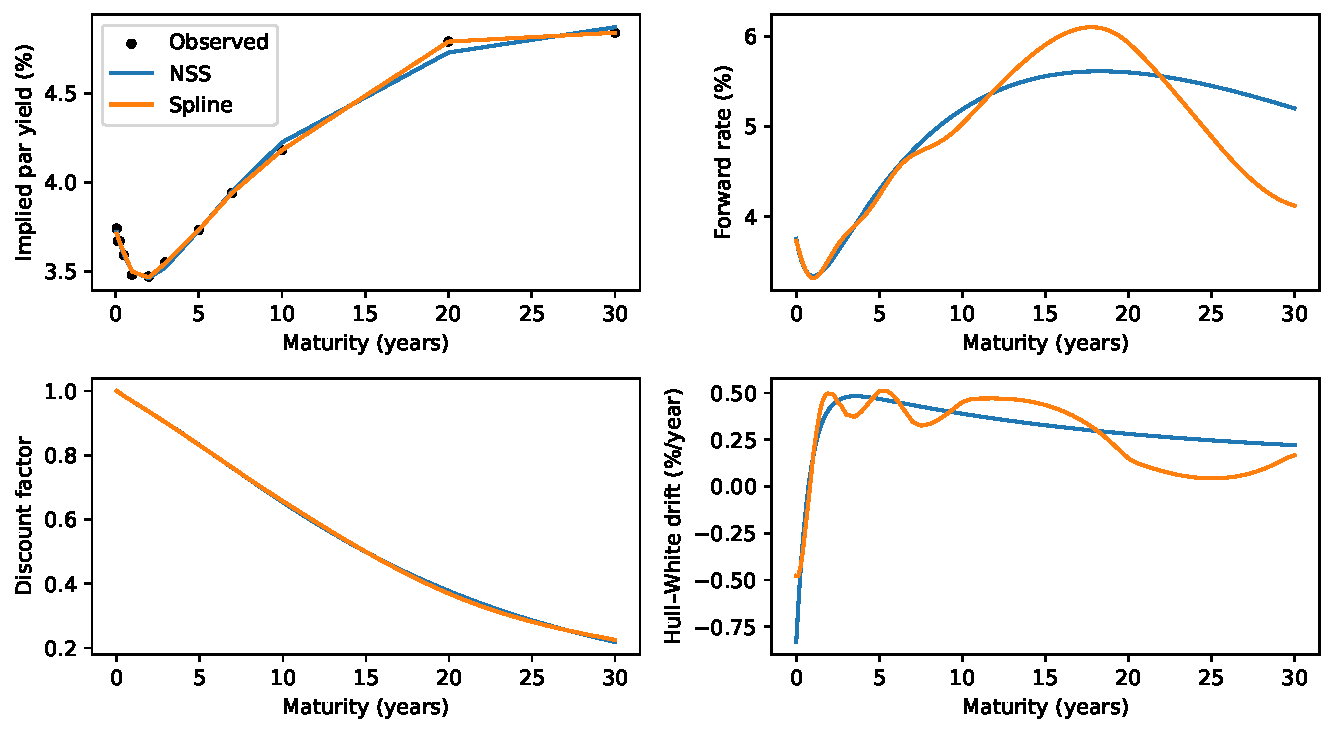
\includegraphics[width=.96\linewidth]{results_nss/curves.pdf}
\caption{\ExampleDate{} 관측·적합 Par Yield, Forward Rate, Discount Factor, Hull--White Drift $\theta(t)$.}
\end{figure}

\textbf{곡선 적합은 Spline이 더 좋았다.}
동일한 관측 Par Yield 기준 중앙값 RMSE가 2.064\,bp로 NSS의 3.482\,bp보다 낮았다. Spline은 만기 구간별 굴곡을 따라갈 수 있다. NSS는 두 감쇠 규모를 공유하는 하나의 함수로 전 만기를 설명하며, 일부 날짜의 곡선 굴곡을 덜 따라갔다. Zero-Rate Node는 기존 Spline 실험에서 추정한 값이므로, 두 방법의 적합도는 관측 Par Yield 기준으로 비교했다.

\clearpage
\subsection{전략별 시장성과}

\begin{table}[!h]
\centering\small
\caption{일별 Gross Hedging P\&L Variance (bp$^2$), 누적 TLT Turnover (기준 IEF 가격 대비 \%), 차감한 Trading Cost (bp).}
\begin{tabular}{lrrrrrr}
\toprule
 & \multicolumn{2}{c}{P\&L Variance} & \multicolumn{2}{c}{Turnover}
 & \multicolumn{2}{c}{Trading Cost}\\
전략 & Spline & NSS & Spline & NSS & Spline & NSS\\
\midrule
\tableinput{results_nss/performance.tex}
\bottomrule
\end{tabular}
\end{table}

\begin{figure}[!h]
\centering
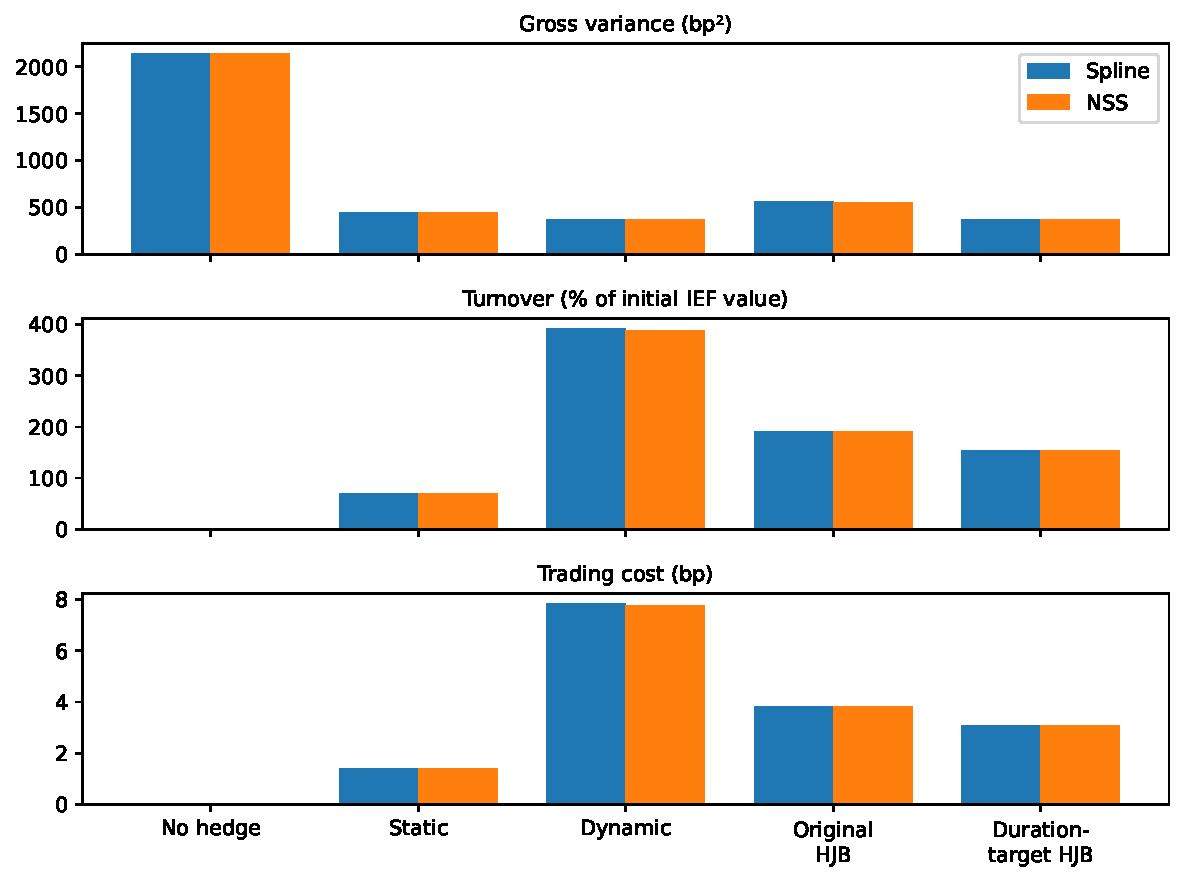
\includegraphics[width=.78\linewidth]{results_nss/metrics.pdf}
\caption{두 곡선 추정법을 적용한 다섯 전략의 P\&L Variance, Turnover, Trading Cost.}
\end{figure}

\textbf{분산은 Dynamic Duration이 가장 낮았다.}
두 곡선에서 모두 약 370\,bp$^2$였다. Duration-Target HJB도 약 371\,bp$^2$를 기록하면서, Dynamic Duration보다 Turnover와 비용을 약 60\% 줄였다. 두 전략은 같은 듀레이션 목표를 사용하고, HJB는 거래를 여러 날에 걸쳐 나눠 조정한다.

\textbf{Original HJB의 분산은 NSS가 약 2\% 낮았다.}
Spline의 564.473\,bp$^2$에서 NSS의 553.226\,bp$^2$로 감소했다. 비용은 둘 다 3.809\,bp였다. 저장된 손익으로 분해하면, TLT 수량 차이에서 생긴 추가 손익의 분산은 $+0.238$\,bp$^2$였고 기존 Spline 손익과의 공분산 항은 $-11.486$\,bp$^2$였다. 이 표본에서는 수량 차이로 생긴 손익이 기존 손익 변동을 일부 상쇄했다. Short Rate 한 요인에 맞춘 두 HJB는 Yield Curve의 기울기나 곡률이 변할 때 잔여 위험이 생길 수 있다.

\clearpage
\subsection{모형별 Original HJB Objective}

\begin{table}[!h]
\centering\small
\caption{각 모형의 Hull--White Risk Exposure로 계산한 Objective Functional ($10^{-6}$ 정규화 손익 제곱).}
\begin{tabular}{lrrrr}
\toprule
전략 & Risk Loss & Trading-Rate Penalty & Terminal Penalty & Total Objective\\
\midrule
\tableinput{results_nss/objective.tex}
\bottomrule
\end{tabular}
\end{table}

Objective Functional은 각 모형에서 사용한 Risk Exposure로 평가했다. 시장성과는 앞 표의 P\&L Variance, Turnover, Trading Cost로 비교한다.

\begin{figure}[!h]
\centering
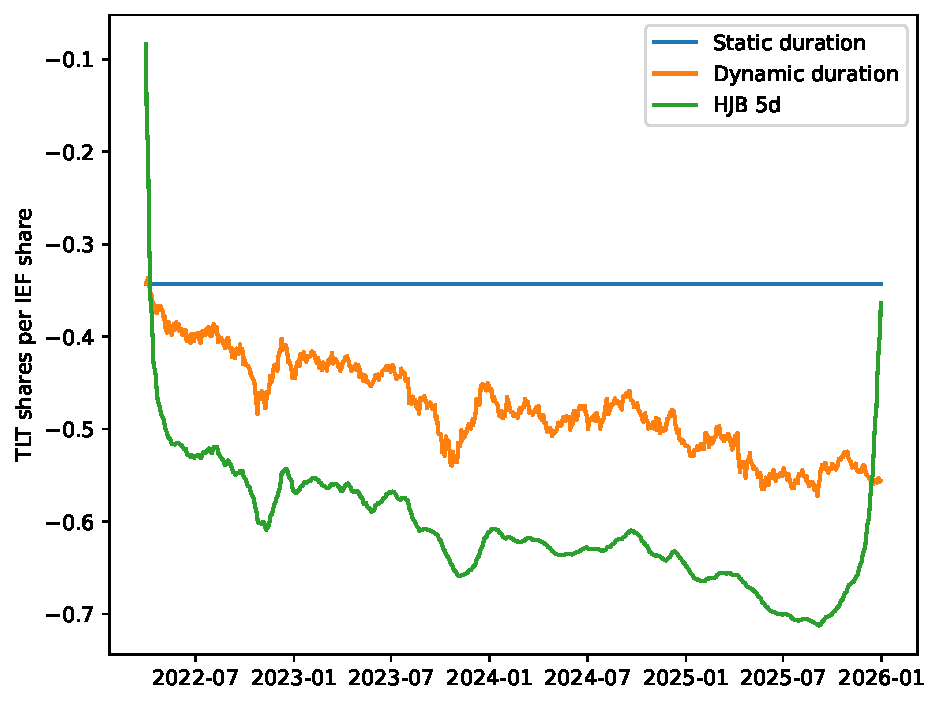
\includegraphics[width=.49\linewidth]{results/position.pdf}
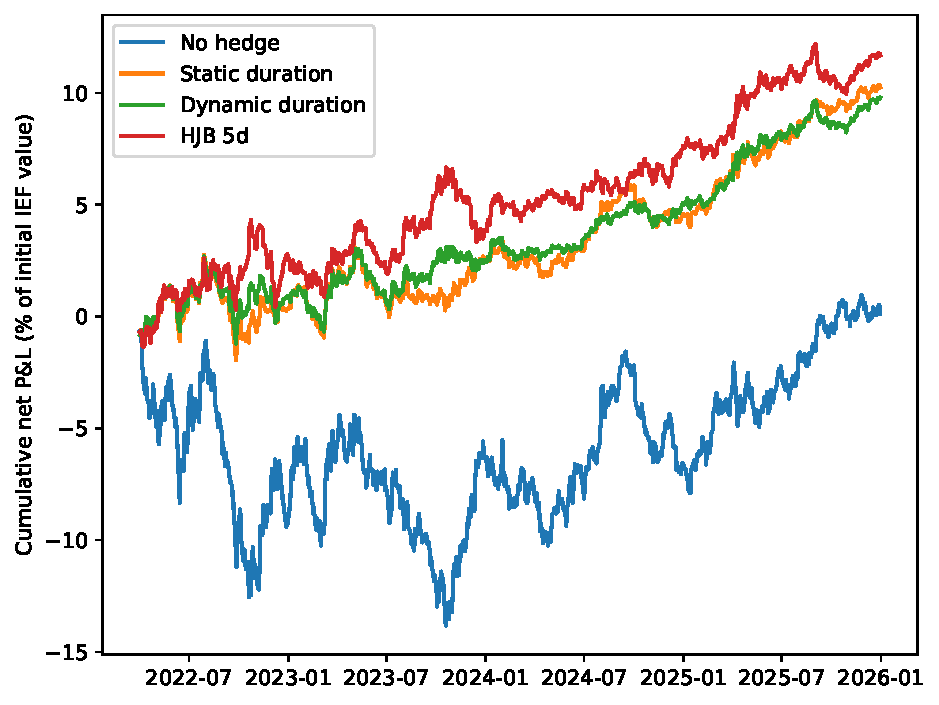
\includegraphics[width=.49\linewidth]{results/pnl.pdf}
\caption{기존 Spline 실험의 TLT 포지션과 Trading Cost 차감 후 Cumulative Hedging P\&L.}
\end{figure}

\subsection{Trading-Rate Penalty 민감도}

\begin{table}[!h]
\centering\small
\caption{기존 Spline HJB의 Trading-Rate Penalty 민감도. Turnover와 Net P\&L은 기준 IEF 가격 대비 비율이다.}
\begin{tabular}{rrrrrrr}
\toprule
설정(일) & $\lambda$ & P\&L SD (bp) & Turnover (\%) & $\int u^2\dif t$ & Penalty & Net P\&L (\%)\\
\midrule
\tableinput{results/penalties.tex}
\bottomrule
\end{tabular}
\end{table}

\begin{figure}[!h]
\centering
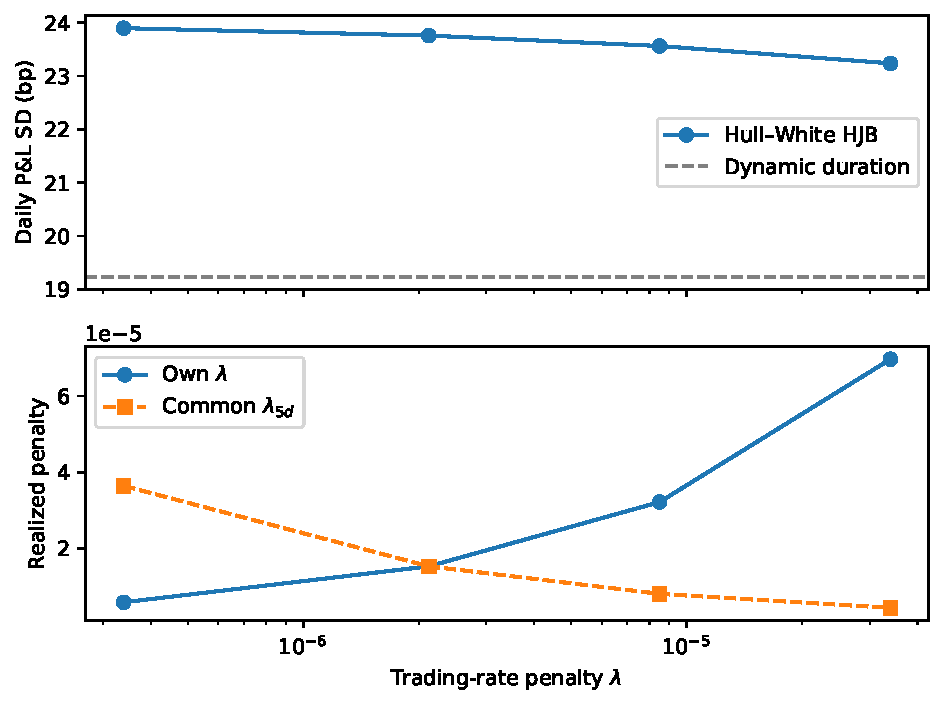
\includegraphics[width=.49\linewidth]{results/sensitivity.pdf}
\caption{Trading-Rate Penalty에 따른 P\&L Standard Deviation과 실현 Trading-Rate Penalty.}
\end{figure}

\clearpage
\begin{thebibliography}{9}
\bibitem{reinsch} Reinsch, C. M. (1967). Smoothing by spline functions.
Numerische Mathematik, 10, 177--183.
\href{https://doi.org/10.1007/BF02162161}{원문}.
\bibitem{svensson} Svensson, L. E. O. (1994). Estimating and interpreting forward interest rates.
IMF Working Papers, 1994/114.
\href{https://doi.org/10.5089/9781451853759.001}{원문}.
\bibitem{hw} Hull, J. and White, A. (1990). Pricing interest-rate-derivative securities.
Review of Financial Studies, 3, 573--592.
\href{https://doi.org/10.1093/rfs/3.4.573}{원문}.
\bibitem{treasury} 미국 재무부.
\href{https://home.treasury.gov/resource-center/data-chart-center/interest-rates}{일별 국채 Par Yield}.
\bibitem{ief} Nasdaq. IEF
\href{https://www.nasdaq.com/market-activity/etf/ief/historical}{종가},
\href{https://www.nasdaq.com/market-activity/etf/ief/dividend-history}{분배금}.
\bibitem{tlt} Nasdaq. TLT
\href{https://www.nasdaq.com/market-activity/etf/tlt/historical}{종가},
\href{https://www.nasdaq.com/market-activity/etf/tlt/dividend-history}{분배금}.
\end{thebibliography}
\end{document}
